% ______________________________________________________________________________
%
%   1DV607 Objectorienterad Analysis och Design med UML
%   Workshop 1 --- "Domain Modeling"
%
%  Author:  Jonas Sjöberg
%           Linnaeus University
%           js224eh@student.lnu.se
%           https://github.com/jonasjberg
%
% License:  Creative Commons Attribution 4.0 International (CC BY 4.0)
%           <http://creativecommons.org/licenses/by/4.0/legalcode>
%           See LICENSE.md for additional licensing information.
% ______________________________________________________________________________


% ______________________________________________________________________________
\section{Analysis}
The analysis is based on the given problem description\ref{probdesc}.
All work has been done by Jonas Sjöberg, without collaborators.


\subsection{Analysis of Requirements for Grade 2}
This analysis delimits the domain model to the following requirements:

\begin{itemize}
  \item \ref{usecase1} Authenticate
  \item \ref{usecase4} Register Boat
  \item \ref{usecase5} Remove Boat
  \item \ref{usecase6} Change Boat
  \item \ref{usecase8} Assign Berths
  \item \ref{usecase10} Manage Calendar Event
  \item \ref{usecase11} List Calendar Events
  \item \ref{usecase12} Show Calendar Event
\end{itemize}


\subsubsection{Domain Model for Grade 2}
\begin{figure}[htbp]
  \centering
  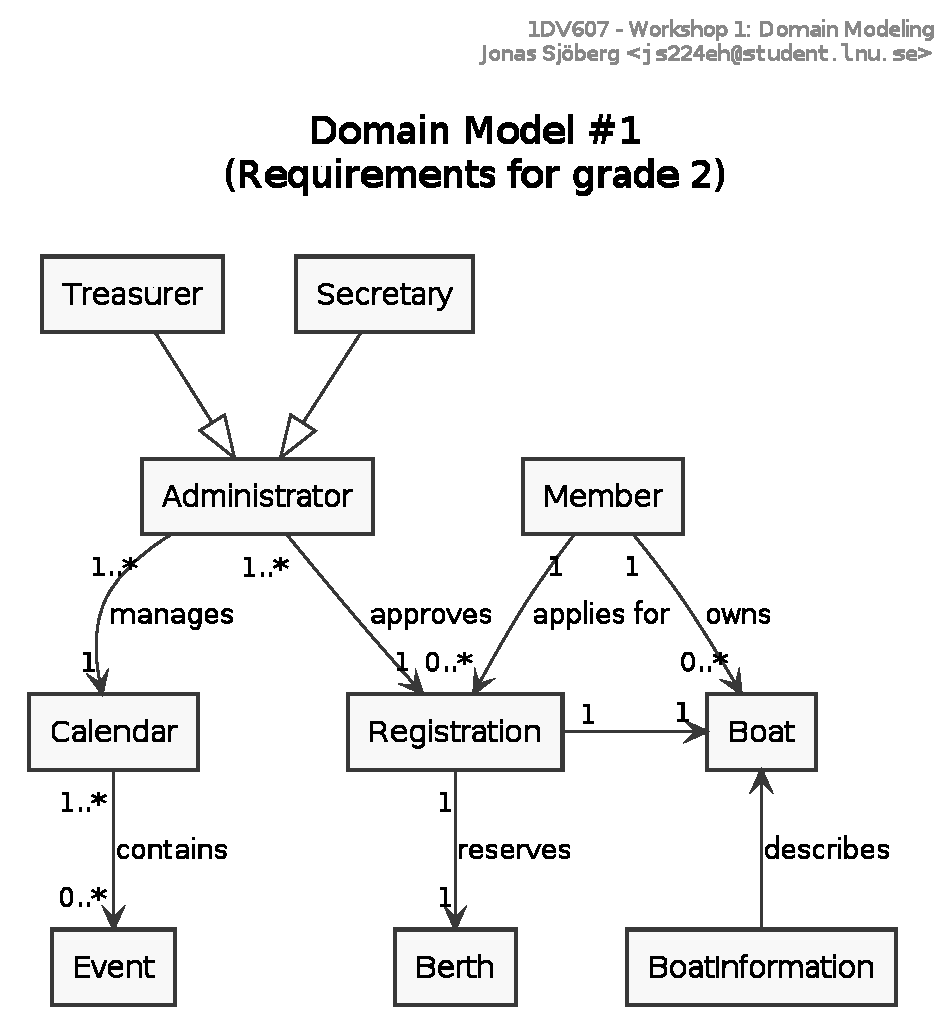
\includegraphics[width=\linewidth]{uml/domain-model_1.eps}
  \caption{UML Domain Model for Grade 2}
  \label{fig:uml-domain1}
\end{figure}

\subsubsection{Notes on the initial domain model}
The first domain model includes the concept of ``AccessControl'', just to
illustrate that the roles of ``Secretary'' and ``Treasurer'' are assumed to be
equivalent and are both treated as a form of ``Administrator''.

The administrators have elevated privileges, as compared to the ``Members''.



\subsection{Analysis of Requirements for Grade 3}
This analysis includes all of the requirements stated in the problem
description \ref{probdesc}.

\subsubsection{Domain Model for Grade 3}
\begin{figure}[htbp]
  \centering
  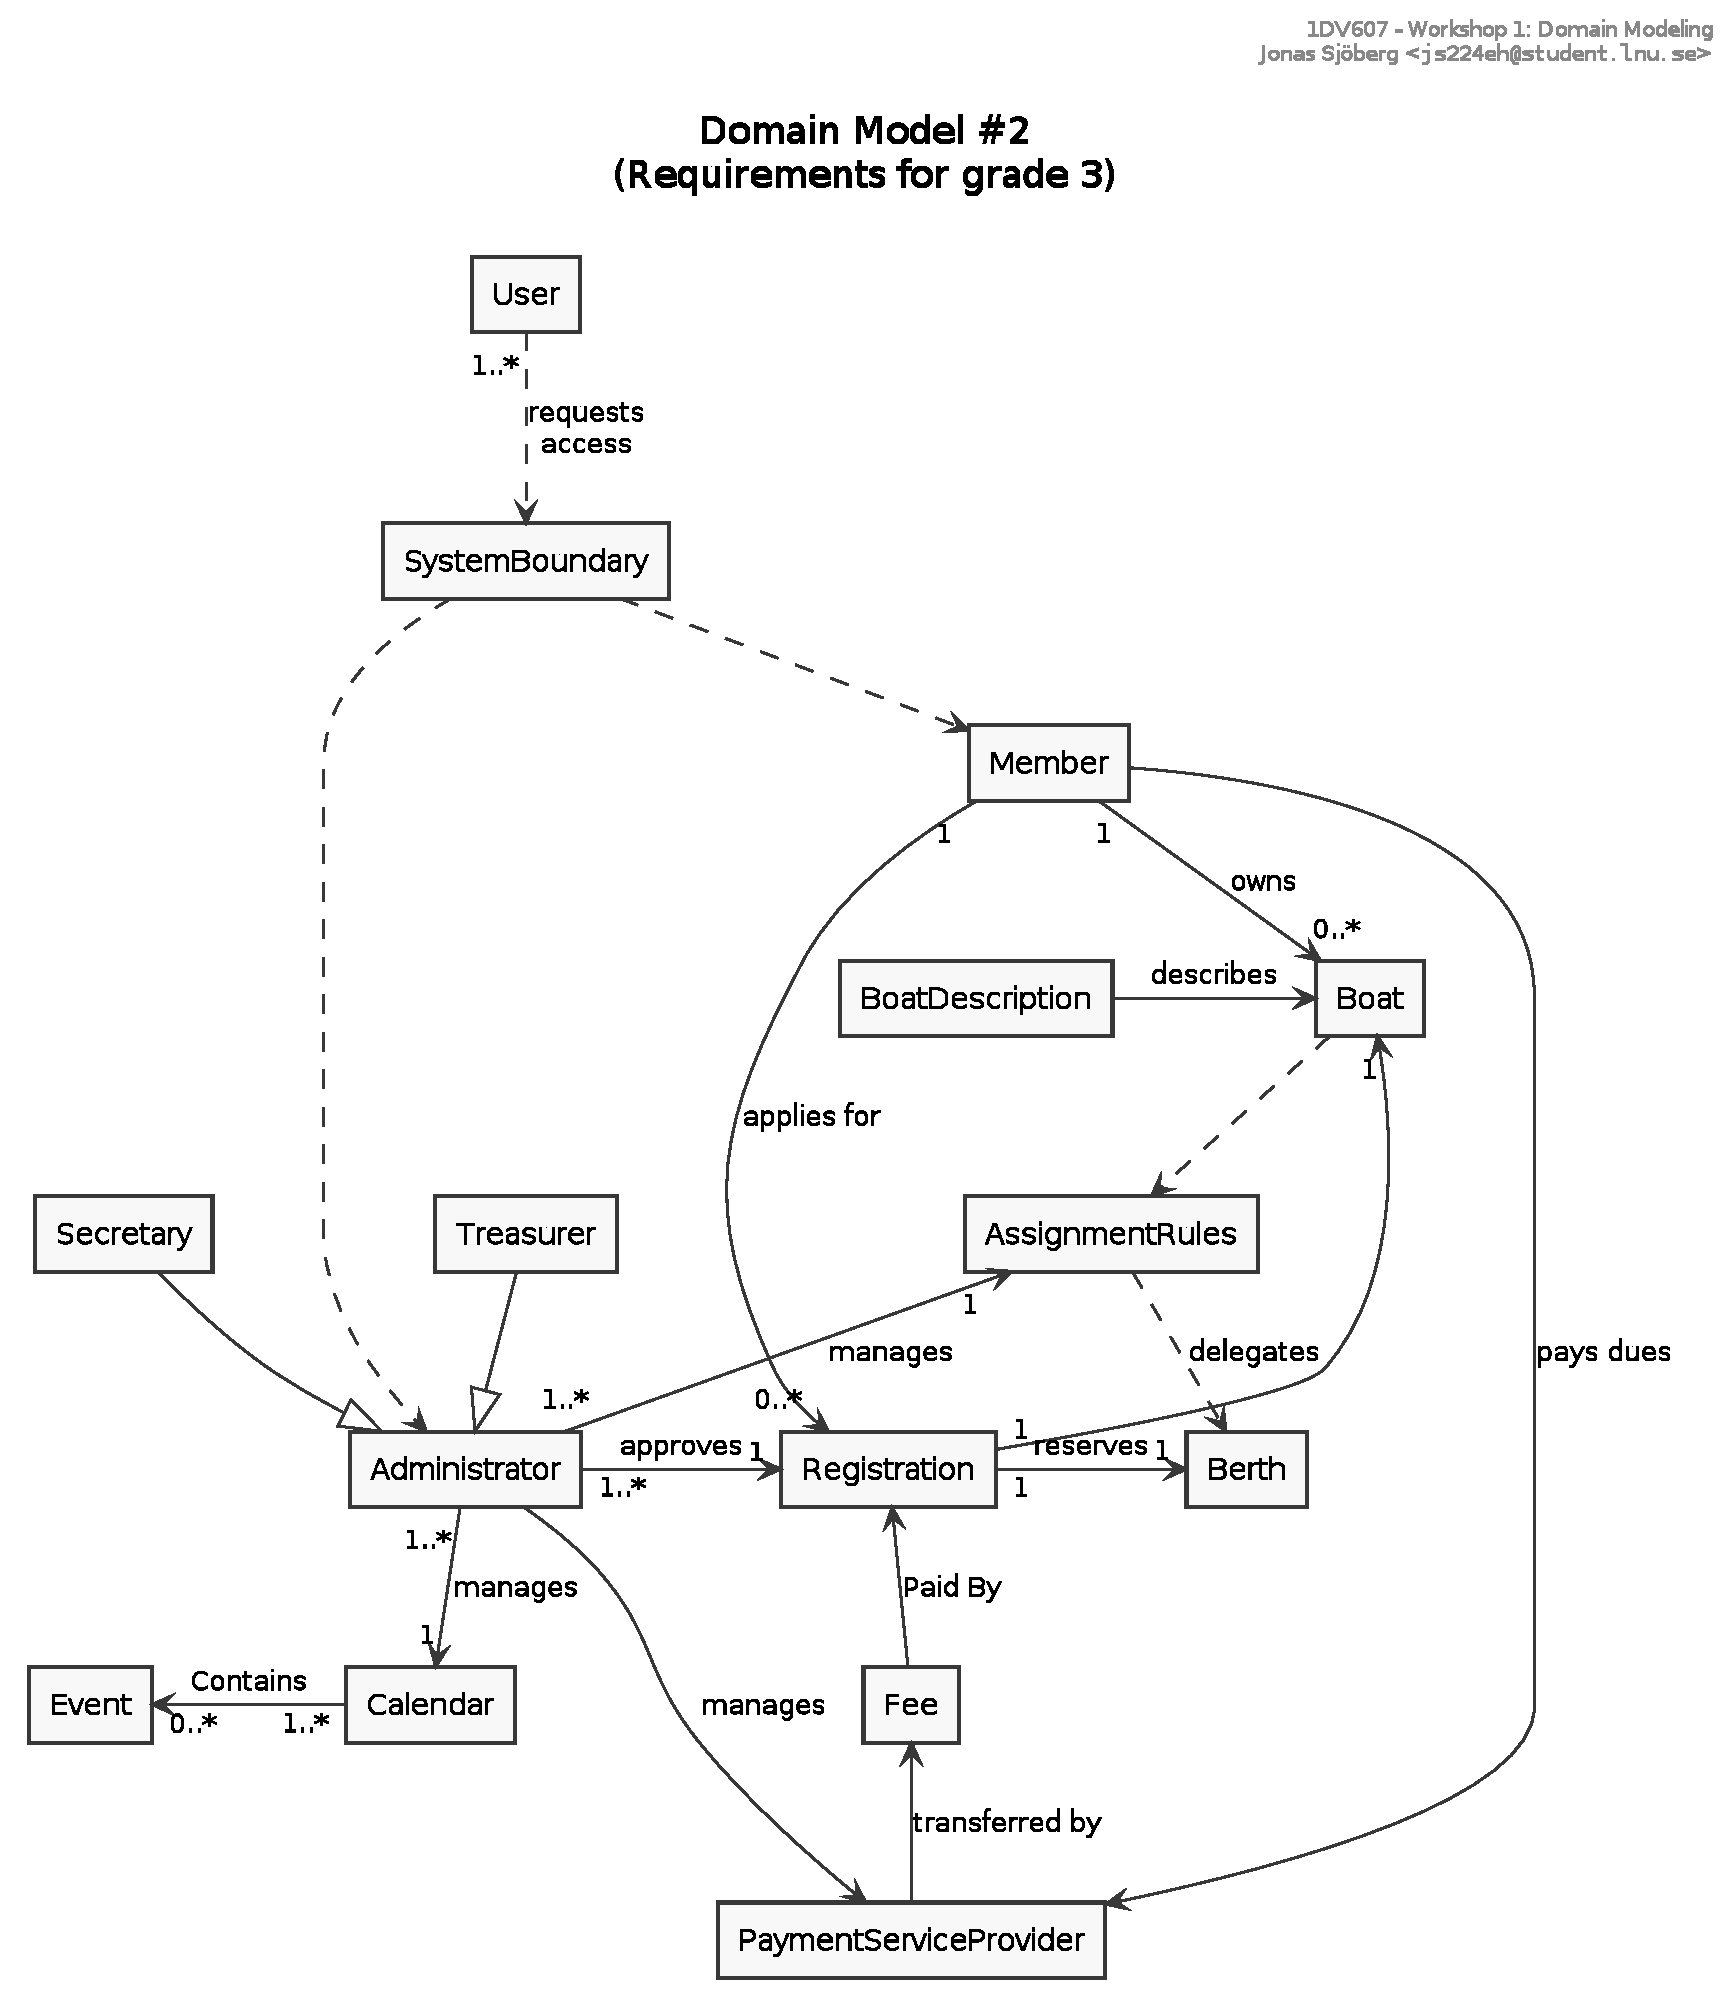
\includegraphics[width=\linewidth]{uml/domain-model_2.eps}
  \caption{UML Domain Model for Grade 3}
  \label{fig:uml-domain2}
\end{figure}

\subsubsection{Notes on the initial domain model}
The biggest change is the introduction of a payment service provider.

Most of the other requirements involve presentation of various data or managing
data in certain ways.  This is restricted to the different user-levels,
administrators should be able to manage invoices, etc.  These requirements
could be modeled with ``description classes'', which have been omitted for
clarity.


